\hsection{Global Optima of the Objective Function}%
%
We now know three key-components of an optimization problem.
We are looking for a candidate solution~$\globalOptimumOf{\solspel}\in\solutionSpace$ that has the best objective value~$\objfOf{\globalOptimumOf{\solspel}}$ for a given problem instance~\instance.
But what is the meaning \inQuotes{best}?%
%
\hsection{Definitions}%
%
Assume that we have a single objective function~$\objf:\solutionSpace\mapsto\realNumbers$ defined over a solution space~$\solutionSpace$.
This objective function is our primary guide during the search and we are looking for its \emph{global optima}.%
%
\begin{definition}[Global Optimum]%
\label{def:globalOptimum}%
If a candidate solution~$\globalOptimumOf{\solspel}\in\solutionSpace$ is a \emph{global optimum} for an optimization problem defined over the solution space~\solutionSpace, then there is no other candidate solution in~\solutionSpace\ which is better.%
\end{definition}%
%
If the objective function is subject to minimization, then each global optimum is a global minimum of the objective function.%
%
\begin{definition}[Global Minimum]%
\label{def:globalMinimum}%
For every \emph{global minimum}~$\globalOptimumOf{\solspel}\in\solutionSpace$ of single-objective optimization problem with solution space~\solutionSpace\ and objective function~$\objf:\solutionSpace\mapsto\realNumbers$ subject to minimization, it holds that $\objfOf{\solspel} \geq \objfOf{\globalOptimumOf{\solspel}} \forall \solspel \in \solutionSpace$.%
\end{definition}%
%
Notice that \cref{def:globalMinimum} does not state that the objective value of~\globalOptimumOf{\solspel} needs to be better than the objective value of all other possible solutions.
The reason is that there may be more than one global optimum, in which case all of them have the same objective value.
Thus, a global optimum is not defined as a candidate solutions better than all other solutions, but as a solution for which no better alternative exists.

The real-world meaning of \inQuotes{globally optimal} is nothing else than \inQuotes{superlative}~\cite{BB2009NO}.
If we solve a \gls{JSSP} for a factory, our goal is to find the \emph{shortest} makespan.
If we try to pack the factory's products into containers, i.e., solve a \gls{BPP},, we look for the packing that needs the \emph{least} amount of containers.
If we solve a vehicle routing problem to serve several customers, then we may either want to serve the \emph{most} customers, use the \emph{least} amount of vehicles, or travel the \emph{shortest} overall distance.
Thus, optimization means searching for such superlatives, as illustrated in \cref{fig:optimization_superlatives}.
Vice versa, whenever we are looking for the cheapest, fastest, strongest, best, biggest or smallest \inQuotes{thing}, then we have an optimization problem at our hands~\cite{KBBDCGJLMPQSVBY2016GLPFOR}.%
%
\begin{figure}%
\centering%
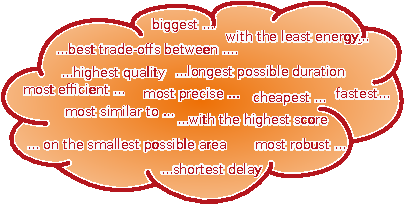
\includegraphics[width=0.7\linewidth]{\currentDir/optimization_superlatives.pdf}%
\caption{Optimization is the search for superlatives~\cite{BB2009NO}.}%
\label{fig:optimization_superlatives}%
\end{figure}%
\endhsection%
%
\begin{definition}[Exact Algorithm]%
An \emph{exact} algorithm guarantees to always find a globally optimal solution for an optimization problem if it is given sufficiently much runtime to complete its computation.%
\end{definition}%
%
At the present state of research, any algorithm guaranteeing to always find the optimal solution of any \NPhard\ optimization problem may require a runtime that is exponential in the \emph{problem scale}.
Very early in this book, in \cref{fig:function_growth}, we saw that exponential growth is very problematic.

This does not mean that exact algorithms \emph{always} need a very long time.
One the one hand, if the problem scale is small, then even an exponential runtime is not very long.
On the other hand, we can imagine a \gls{TSP} instance with millions of cities which all are located on a circle.
Or we can imagine a \gls{BPP} where all the items to be packed have the same size.
Such problem instances would be very easy to solve, regardless of their scale.

However, for \NPhard\ problems, there is a correlation between the size~$|\solutionSpace|$ of the solution space~\solutionSpace\ and the runtime an \emph{exact} algorithm may need.%
%
\begin{definition}[Heuristic Algorithm]%
A \emph{heuristic} algorithm does \emph{not guarantee} to find a globally optimal solution, but it will find one solution of hopefully good quality within a hopefully shorter runtime.%
\end{definition}%
%
%
\hsection{Example: Job Shop Scheduling}%
%
For the \gls{JSSP}, there exists a simple and fast algorithm that can find the optimal schedules for problem instances with exactly $\jsspMachines=2$~machines \emph{and} where all $\jsspJobs$~jobs need to be processed by the two machines in exactly the same order~\cite{J1954OTATSPSWSTI}.
If our application always falls into such a special case of the problem we are dealing with, we may be lucky to find an efficient way to always solve it to optimality.

The general version of the \gls{JSSP}, however, is indeed \NPhard~\cite{LLRKS1993SASAAC,CPW1998AROMSCAAA}, meaning that we cannot expect to solve it to global optimality in reasonable time.
For the \gls{JSSP}, the problem scale is defined by the numbers of machines~\jsspMachines\ and jobs~\jsspJobs\ involved.
In \cref{tbl:jsspSolutionSpaceSizeTable} we saw that the size of the solution space~\solutionSpace\ grows very quickly with~\jsspMachines\ and~\jsspJobs.
And so will the runtime of exact methods.

\begin{figure}%
\centering%
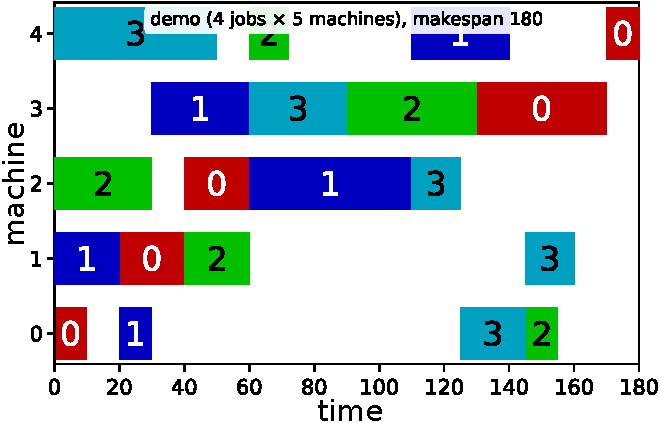
\includegraphics[width=0.55\linewidth]{\currentDir/gantt_demo_opt_with_makespan.pdf}%
\caption{The optimal solution of the \instStyle{demo} instance given in \cref{fig:jssp_demo_instance}.}%
\label{fig:gantt_demo_opt_with_makespan}%
\end{figure}

For small instances of the \gls{JSSP}, however, we can still find the optimal solution by simply enumerating all possible Gantt charts and picking the one with shortest makespan, i.e., the best objective value.
In \cref{fig:gantt_demo_opt_with_makespan}, we illustrate the optimal solution for our small \instStyle{demo} instance that was discovered this way.
This method will obviously not work on bigger problems.%
%
\ruleOfThumb{scale1}{Algorithms working well on small-scale toy problem instances do not necessarily work well on reasonably-sized or large-scale instances.}%
%
From this we can immediately conclude the following rule, which is an important basic wisdom that we must never forget throughout our career:%
%
\ruleOfThumb{scale2}{In order to correctly understand the performance and behavior of an algorithm, testing it on small-scale instances is insufficient.}%
%
\endhsection%
%
\hsection{Summary}%
In this section, we learned a bit more about the nature of optimization.
In particular, we formalized the concept of the best-possible solutions, the global optima~\globalOptimumOf{\solspel} in the solution space~\solutionSpace\ based on the objective function~\objf.

We also re-iterated the reason why we need metaheuristic optimization:
Many optimization problems are \NPhard\ and solving them to guaranteed optimality will often take too much time.
Therefore, developing a good (meta-)heuristic algorithm, which cannot provide \emph{guaranteed} optimality but will give close-to-optimal solutions in practice, is a good choice.

We also implicitly learned that, despite being \NPhard, we can solve small-scale instances of the \gls{JSSP} to optimality.
But we can do this only for the really small instances.
And this is the case for many of the well-known optimization problems.%
\endhsection%
\endhsection%
%
